% -----------------------------------------------------------------------------
% Latex Template for Wuhan University Thesis
%
% Ack to Huang Zhenghua (http://aff.whu.edu.cn/huangzh/)
%
% Modified by iamywang
% Date: Jan 29, 2024
% -----------------------------------------------------------------------------

% 选项 [forprint]: 交付打印时, 加上此选项, 以消除链接文字之彩色, 避免打印偏淡.
% 选项 [forlib]: 提交给图书馆的电子版, 需要加上选项 forlib, 以消除空白页和彩色链接.
\documentclass[forlib,AutoFakeBold=2]{WHUPhd}
\usepackage{gbt7714}
\usepackage{listings}
\usepackage{multirow}
\usepackage{setspace}
\usepackage{titletoc}
\usepackage{pdfpages}

\hypersetup{hidelinks}

\lstset{
language=C++,
showstringspaces=false,
basicstyle=\small\ttfamily,
rulesepcolor=\color{gray},
breaklines=true,
keywordstyle=\color{purple}\bfseries,
commentstyle=\color{gray!80!black},
stringstyle=\color{blue!80!black},
frame=single,
flexiblecolumns=true,
lineskip={-1pt}
}

\begin{document}

% 封面表头信息
\fenleihao{TP309}
\miji{}
\UDC{}
\bianhao{10486}

% 封面内容
\title{XXX关键技术研究}
\Etitle{Research on Key Techniques for XXXX}
\author{X\hfill X\hfill X}
\Eauthor{XXX}
\Csupervisor{X\hfill X\hfill \hfill 教\hfill 授}
\Esupervisor{Prof.~XX}
\Cmajor{网\hfill 络\hfill 空\hfill 间\hfill 安\hfill 全}
\Emajor{Cyberspace Security}
\Cspeciality{X\hfill X\hfill X\hfill X}
\Especiality{XXXX}
\Schoolname{School of Cyber Science and Engineering}
\date{二〇二四年一月}
\Edate{Jan 2024}

\pdfbookmark[0]{封面}{title}
\maketitle

% 英文封面
% -----------------------------------------------------------------------------
% Latex Template for Wuhan University Thesis
%
% Ack to Huang Zhenghua (http://aff.whu.edu.cn/huangzh/)
%
% Modified by iamywang
% Date: Jan 29, 2024
% -----------------------------------------------------------------------------

\thispagestyle{empty}
\renewcommand{\baselinestretch}{1.5}  %下文的行距
\vspace*{0.5cm}

\begin{center}{\zihao{2} \the\Etitle \par}\end{center}

\vfill

\begin{center}
\zihao{4}
% 表格第二列0.5cm
\setlength{\tabcolsep}{0pt}
\begin{tabular}{rcl}
\makebox{Candidate}  & \makebox[0.5cm][c]{:}  & \makebox{\the\Eauthor}      \\
\makebox{Supervisor} & \makebox[0.5cm][c]{:}  & \makebox{\the\Esupervisor}  \\
\makebox{Major}      & \makebox[0.5cm][c]{:}  & \makebox{\the\Emajor}       \\
\makebox{Speciality} & \makebox[0.5cm][c]{:}  & \makebox{\the\Especiality}
\end{tabular}

\vspace*{2cm}
\begin{center}
  \iflib % 向图书馆提交电子文档, 使用黑白校徽.
  
\includegraphics[height=4cm]{whulogo.eps}       %%  黑白的. 很小, 只有 10k.
  \else
  \ifprint % 文档打印, 使用黑白校徽.
  
\includegraphics[height=4cm]{whulogo.eps}       %%  黑白的.
  \else
  
\includegraphics[height=4cm]{whulogo.eps}       %%  彩色的.
  \fi
  \fi
\end{center}


\zihao{-2}
\the\Schoolname\\
{WUHAN UNIVERSITY}

\vspace*{1.0cm}

\the\Edate

\end{center}
%%%%%%%--判断是否需要空白页-----------------------------
  \iflib
  \else
  \newpage
  \thispagestyle{empty}
  \cleardoublepage
  \fi
%%%%%%%-------------------------------------------------
{\pagestyle{empty}
%%%--- 加入``郑重声明'' --- %%%%%%%%%%%%%%%%%
% -----------------------------------------------------------------------------
% Latex Template for Wuhan University Thesis
%
% Ack to Huang Zhenghua (http://aff.whu.edu.cn/huangzh/)
%
% Modified by iamywang
% Date: Jan 29, 2024
% -----------------------------------------------------------------------------

\newpage
\vspace*{20pt}
\begin{center}{\zihao{-2}\heiti 论文原创性声明}\end{center}
\par\vspace*{30pt}
\renewcommand{\baselinestretch}{2}
{\zihao{4} \songti %
本人郑重声明:所呈交的学位论文,是本人在导师指导下,独立进行研究工作所取得的研究成果。
除文中已经标明引用的内容外,本论文不包含任何其他个人或集体已发表或撰写的研究成果。
对本文的研究做出贡献的个人和集体,均已在文中以明确方式标明。
本声明的法律结果由本人承担。

\vskip2cm

\hspace*{4cm}学位论文作者(签名):\hspace{4cm} \hfill \\[1cm]
\hspace*{10cm}年 \hfill  月 \hfill 日\hspace{1cm}\hfill\par}

%%%%%%%--判断是否需要空白页-----------------------------
  \iflib
  \else
  \newpage
  \cleardoublepage
  \fi
%%%%%%%-------------------------------------------------
\renewcommand{\baselinestretch}{1.5}
\small\normalsize
%%%%%%%%%%%%%%%%%
%%% ---加入``武汉大学学位论文使用授权协议书'' ---  %%%%%%
% -----------------------------------------------------------------------------
% Latex Template for Wuhan University Thesis
%
% Ack to Huang Zhenghua (http://aff.whu.edu.cn/huangzh/)
%
% Modified by iamywang
% Date: Jan 29, 2024
% Updated: Apr 13, 2024
% -----------------------------------------------------------------------------

\newpage
\vspace*{20pt}
\thispagestyle{empty}
\begin{center}{\zihao{4}\heiti \bfseries 武汉大学学位论文使用授权协议书}\end{center}

\vspace*{4pt}

\begin{center}{\zihao{-5}(一式两份,一份论文作者保存,一份留学校存档)}\end{center}

\vspace*{4pt}

本学位论文作者愿意遵守武汉大学关于保存、使用学位论文的管理办法及规定,
即:学校有权保存学位论文的印刷本和电子版,并提供文献检索与阅览服务;
学校可以采用影印、缩印、数字化或其它复制手段保存论文;
在以教学与科研服务为目的前提下,学校可以在校园网内公布部分或全部内容。

一、在本论文提交当年,同意在校园网内以及中国高等教育文献保障系统(CALIS)、高校学位论文系统提供查询及前十六页浏览服务。

二、在本论文提交~$\Box$~当年/~$\Box$~一年/~$\Box$~两年/~$\Box$~三年以后,
同意在校园网内允许读者在线浏览并下载全文,学校可以为存在馆际合作关系的兄弟高校用户提供文献传递服务和交换服务。
(保密论文解密后遵守此规定)

\vskip 0.8cm

论文作者(签名):\raisebox{-1ex}{\underline{\makebox[3.54cm][c]{}}}
\vskip 0.8cm

学\qquad 号:\raisebox{-1ex}{\underline{\makebox[5cm][c]{}}}
\vskip 0.8cm

学\qquad 院:\raisebox{-1ex}{\underline{\makebox[5cm][c]{}}}

\vskip 1cm
\begin{flushright}
日期:\hskip2cm 年\hskip1.2cm 月\hskip1.2cm 日
\end{flushright}

%%%%%%%%%%%%%%%%%%
%%%%%%%%%%%%%%%%%%%%%%%%%%%%%%%
}

%%%%%%%%%%%%%%%%%%%%%%%%%%%%%%%
%%% ------------------- 论文创新点----------------------- %%%
%%%%%%%%%%%%%%%%%%%%%%%%%%%%%%%

\newpage\vspace*{20pt}\thispagestyle{empty}
\begin{center}{\zihao{-2}\heiti 论文创新点}\end{center}
\par\vspace*{30pt}
\baselineskip=20pt

%%%%%%%%%%%%%%%%%%%%%%%%%%%%%%%
%%%%%%%--请勿删除以下内容 -------------------------------%
%%%%%%%--判断是否需要空白页-----------------------------%
  \iflib
  \let\cleardoublepage\clearpage
  \else
  \newpage
  \thispagestyle{empty}
  \cleardoublepage
  \fi
%%%%%%%---------------------------------------------------%


% 目录页面样式设置为含有页眉
\frontmatter
\pagenumbering{Roman}
\pagestyle{fancy}
\fancyfancy

% 目录页面样式设置为不含有页眉
% \frontmatter
% \pagenumbering{Roman}
% \pagestyle{oldplain}

% 目录样式
\titlecontents{chapter}[0em]{\bfseries}{\contentspush{\thecontentslabel \quad}}{}{\titlerule*[4pt]{.}\contentspage}
\titlecontents{section}[1em]{}{\contentspush{\thecontentslabel \quad}}{}{\titlerule*[4pt]{.}\contentspage}
\titlecontents{subsection}[2.5em]{}{\contentspush{\thecontentslabel \quad}}{}{\titlerule*[4pt]{.}\contentspage}
\makeatletter
\def\@dotsep{0.5}
\makeatother

% 目录
\pdfbookmark[0]{目录}{toc}
\begin{spacing}{1.5}
\tableofcontents
\end{spacing}
\newpage

% 插图索引
\renewcommand*{\addvspace}[1]{}
\let\oldnumberline\numberline
\renewcommand{\numberline}{\figurename~\oldnumberline}
\makeatletter
\renewcommand*\l@figure{\@dottedtocline{1}{0em}{2.5em}}
\makeatother
\begin{spacing}{1.5}
\listoffigures
\end{spacing}
\newpage

% 表格索引
\renewcommand{\numberline}{\tablename~\oldnumberline}
\makeatletter
\renewcommand*\l@table{\@dottedtocline{1}{0em}{2.5em}}
\makeatother
\begin{spacing}{1.5}
\listoftables
\end{spacing}
\cleardoublepage

% 中英文缩略语对照表
% -----------------------------------------------------------------------------
% Latex Template for Wuhan University Thesis
%
% Ack to Huang Zhenghua (http://aff.whu.edu.cn/huangzh/)
%
% Modified by iamywang
% Date: Jan 29, 2024
% -----------------------------------------------------------------------------

\chapter{中英文缩略语对照表}

\begin{center}
\renewcommand\arraystretch{1.5}
\setlength{\tabcolsep}{4pt}
\begin{tabular}{p{0.1\linewidth}p{0.5\linewidth}p{0.3\linewidth}}
AES & Advanced Encryption Standard & 高级加密标准 \\
API & Application Programming Interface & 应用程序编程接口 \\
ARM & Advanced RISC Machine & 高级精简指令集机器 \\
ASLR & Address Space Layout Randomization & 地址空间布局随机化 \\

BHB & Branch History Buffer & 分支历史缓冲区 \\
BHI & Branch History Injection & 分支历史注入 \\
BPU & Branch Prediction Unit & 分支预测单元 \\
BRB & Branch Retention Buffer & 分支保留缓冲区 \\
BTB & Branch Target Buffer & 分支目标缓冲区 \\

CNN & Convolutional Neural Network & 卷积神经网络 \\
CPU & Central Processing Unit & 中央处理器 \\
CVE & Common Vulnerabilities and Exposures & 通用漏洞披露 \\
\end{tabular}
\end{center}


% 摘要
% -----------------------------------------------------------------------------
% Latex Template for Wuhan University Thesis
%
% Ack to Huang Zhenghua (http://aff.whu.edu.cn/huangzh/)
%
% Modified by iamywang
% Date: Jan 29, 2024
% -----------------------------------------------------------------------------

%%%%%%%%%%%%%%%%%%%%%%%
%%% ------------ 中文摘要 ---------------%%%
%%%%%%%%%%%%%%%%%%%%%%%
\begin{cnabstract}
摘要。
\end{cnabstract}
\vspace{1em}\par\vfill

%%%--------- 关键词 -------- %%%
\cnkeywords{侧信道攻击}

%%%%%%%%%%%%%%%%%%%%%%%


%%%%%%%%%%%%%%%%%%%%%%%
%%% ------------ 英文摘要 ---------------%%%
%%%%%%%%%%%%%%%%%%%%%%%
\begin{enabstract}
Abstract.
\end{enabstract}
\vspace{1em}\par\vfill

%%%------ 英文关键词 ------- %%%
\enkeywords{Side-Channel Attack}


% 正文样式
\mainmatter
\renewcommand{\baselinestretch}{1.5}
\renewcommand{\arraystretch}{1.5}
\baselineskip=20pt
\CTEXsetup[nameformat={\normalfont\zihao{-2}\heiti\raggedright},
titleformat={\normalfont\zihao{-2}\heiti\raggedright},
number={\arabic{chapter}},name={,},afterskip={4pt},beforeskip={-28pt}]{chapter}
\pagestyle{fancy}
\fancyfancy

% 正文
% -----------------------------------------------------------------------------
% Latex Template for Wuhan University Thesis
%
% Ack to Huang Zhenghua (http://aff.whu.edu.cn/huangzh/)
%
% Modified by iamywang
% Date: Jan 29, 2024
% -----------------------------------------------------------------------------

\chapter{绪论}\label{chap1}

\section{研究背景与意义}
随着XXXX\cite{aciiccmez2010new}发展,

XXXX

进一步XXXXXX。

\section{国内外研究现状}
XXXX
\subsection{XXXX技术研究现状}
XXXX
\subsection{XXXX技术研究现状}
XXXX
\subsection{XXXX技术研究现状}


% -----------------------------------------------------------------------------
% Latex Template for Wuhan University Thesis
%
% Ack to Huang Zhenghua (http://aff.whu.edu.cn/huangzh/)
%
% Modified by iamywang
% Date: Jan 29, 2024
% -----------------------------------------------------------------------------

\chapter{相关工作综述}\label{chap2}

% -----------------------------------------------------------------------------
% Latex Template for Wuhan University Thesis
%
% Ack to Huang Zhenghua (http://aff.whu.edu.cn/huangzh/)
%
% Modified by iamywang
% Date: Jan 29, 2024
% Updated: Apr 13, 2024
% -----------------------------------------------------------------------------

\chapter{内存安全问题研究}\label{chap3}

从计算机体系结构的角度来说,内存安全违规(memory safety violation)一般分为两大类:

(1)时间违规(temporal violation):典型代表为Use-After-Free(UAF)漏洞,即在释放内存后,再次对该内存进行访问。

(2)空间违规(spatial violation):典型代表为栈溢出(stack overflow)漏洞,即在栈上分配的内存空间不足以存放当前的数据。

而面向返回编程(Return-Oriented Programming,ROP)、面向跳转编程(Jump-Oriented Programming,JOP)和面向调用编程(Call-Oriented Programming,COP)都是基于空间违规的攻击手段,本文将从攻击基本原理、现有芯片级对策和思考三个方面来介绍ROP/JOP/COP。

而ROP攻击产生的一大原因是因为,现代操作系统为了防止攻击者在栈上发起代码注入漏洞,采用了$W \oplus X$的内存保护机制,即栈上的内存空间只能执行,不能写入。因此,攻击者在栈上发起代码注入漏洞时,只能通过覆盖返回地址来控制程序的执行流程,而这种攻击手段就是ROP。
% -----------------------------------------------------------------------------
% Latex Template for Wuhan University Thesis
%
% Ack to Huang Zhenghua (http://aff.whu.edu.cn/huangzh/)
%
% Modified by iamywang
% Date: Jan 29, 2024
% Updated: Apr 13, 2024
% -----------------------------------------------------------------------------

\chapter{硬件级安全机制研究}\label{chap4}

\section{Intel CET安全机制分析}

Intel CET(Control-Flow Enforcement Technology)是Intel新推出的一项新的硬件级对策,其主要目的是防止攻击者通过ROP/JOP/COP等攻击手段来劫持控制流。
对于ROP攻击的防护,其基本思想与影子栈(shadow stack)类似,即由操作系统在内存中复制一份程序的内存栈或者是仅仅保留控制流跳转地址。然后,这个影子栈无法由正常的store、load指令进行控制,只能通过专门的指令来进行控制。因此,即使攻击者覆盖了软件栈上的返回地址,但是由于影子栈中仍然保存着原始的跳转地址,因此检查失败后会通过抛出异常来终止程序的执行。
对于JOP/COP攻击的防护,Intel提出一种叫做IBT(Indirect Branch Tracking)的技术,其基本思想是通过编译器在合理的间接跳转中⽤新的指令做标记,然后程序执行时会检查下一条指令是否为新添加的指令(endbr),如果不是则会抛出\#CP异常。

\section{ARM PAC安全机制分析}

ARM PAC(Pointer Authentication)是ARMv8.3引入的一项新的硬件级对策,其主要通过对指针进行鉴权来防止攻击者通过ROP/JOP/COP等攻击手段来劫持控制流。
这种防护方法的基本原理是,利用64位地址空间中暂时空闲的高16位来存放指针的鉴权结果(MAC码),然后在每次指针使用前,都会对指针进行鉴权,如果鉴权失败,则会抛出异常来终止程序的执行。
% -----------------------------------------------------------------------------
% Latex Template for Wuhan University Thesis
%
% Ack to Huang Zhenghua (http://aff.whu.edu.cn/huangzh/)
%
% Modified by iamywang
% Date: Jan 29, 2024
% Updated: Apr 13, 2024
% -----------------------------------------------------------------------------

\chapter{安全架构设计关键技术研究}\label{chap5}

\section{ZeRØ安全架构设计}

ZeRØ~\cite{ziad2021zero}提出了独特的内存指令和新颖的元数据编码方案来保护代码和数据指针,仅仅只需要微小的微架构变化。ZeRØ在SPEC CPU2017基准上的性能开销为零,VLSI测量显示了低功率和面积开销。

\begin{figure}[h!]
\centering
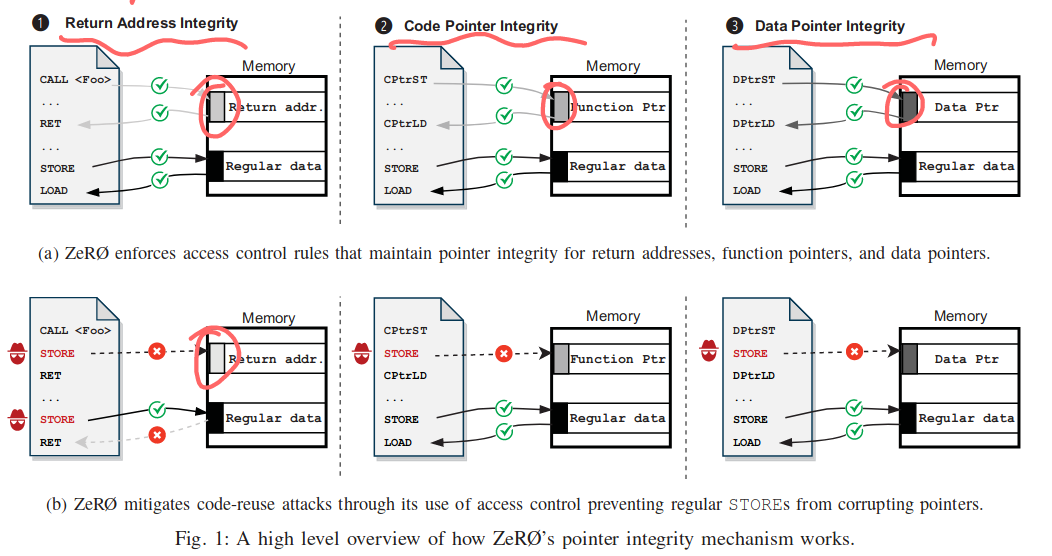
\includegraphics[width=0.8\linewidth]{fig5-1.png}
\caption{ZeRØ设计框架}
\label{fig5.1}
\end{figure}

\section{No-FAT安全架构设计}

No-FAT~\cite{ziad2021no}将内存分配大小(例如malloc大小)作为一个架构特征,来克服传统内存安全方法的许多棘手问题,例如与不安全软件的兼容性和显著的性能下降。No-FAT在SPEC CPU2017基准测试中产生了8\%的开销,VLSI测量显示了低功率和面积开销。

\begin{figure}[h!]
\centering
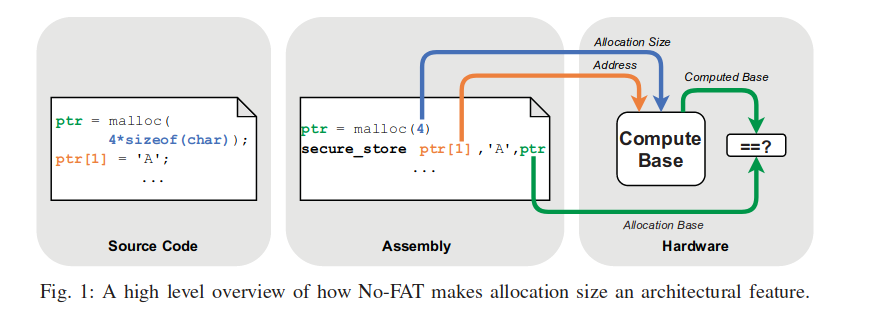
\includegraphics[width=0.8\linewidth]{fig5-2.png}
\caption{No-FAT设计框架}
\label{fig5.2}
\end{figure}
% -----------------------------------------------------------------------------
% Latex Template for Wuhan University Thesis
%
% Ack to Huang Zhenghua (http://aff.whu.edu.cn/huangzh/)
%
% Modified by iamywang
% Date: Jan 29, 2024
% -----------------------------------------------------------------------------

\chapter{针对XXXXX的XXXXX}\label{chap6}

% -----------------------------------------------------------------------------
% Latex Template for Wuhan University Thesis
%
% Ack to Huang Zhenghua (http://aff.whu.edu.cn/huangzh/)
%
% Modified by iamywang
% Date: Jan 29, 2024
% -----------------------------------------------------------------------------

\chapter{总结与展望}\label{chap7}

\section{本文总结}

\section{未来工作展望}


% 参考文献
\cleardoublepage\phantomsection
\addcontentsline{toc}{chapter}{参考文献}
\renewcommand{\bibfont}{\zihao{5}}
\setlength{\bibsep}{0pt}
\bibliographystyle{gbt7714-numerical}
\bibliography{bibs/ref1, bibs/ref2, bibs/ref3, bibs/ref4, bibs/ref5, bibs/ref6, bibs/ref7}

% 科研成果和致谢
\backmatter
% -----------------------------------------------------------------------------
% Latex Template for Wuhan University Thesis
%
% Ack to Huang Zhenghua (http://aff.whu.edu.cn/huangzh/)
%
% Modified by iamywang
% Date: Jan 29, 2024
% -----------------------------------------------------------------------------

\reseachresult

\subsection*{作者简历}

XXX(19XX—),男,湖北武汉人,武汉大学XXX学院博士研究生

研究方向:XXXX

2021年9月——至今,武汉大学,XXXX

\subsection*{学术论文}
\begin{enumerate}[{[}1{]}]

\item \textbf{XXX}, XXX*.
Title.
\textit{Jounral/Conference}\\
\textbf{(CCF-A类会议,对应论文第~\ref{chap3}~章)}
\end{enumerate}

\subsection*{发明专利}
\begin{enumerate}[{[}1{]}]
\item 一种XXXX方法及系统,
发明人:XXX、\textbf{XXX},申请中,
申请号:XXXXX,申请日:XXXX年XX月XX日
\end{enumerate}

\subsection*{获奖情况}
\begin{enumerate}[{[}1{]}]
\item 武汉大学XXXX奖学金,一等奖,2021
\item 武汉大学XXXX奖学金,一等奖,2022
\end{enumerate}

\acknowledgement

%%%%%%%%%%%%%%%%%%%%%%%%%%%%%%%%%%%%%%%
%%%%%%%--判断是否需要空白页-----------------------------
  \iflib
  \else
  \newpage
  %\thispagestyle{empty}`
  \cleardoublepage
  \fi
%%%%%%%-------------------------------------------------


\cleardoublepage
\end{document}
